% =====================================================================
%  Parts I and II: the Laplacian and the modularity matrix under unit
%  degree; the market factor as an implicit null model.
%  Proposal "Modularity Matrix Approach for Graph Learning?" (Oct 2026).
%  Self-contained: no .bib, no \includegraphics, no external data.
%  Compiles on Overleaf as-is, and locally with:
%      tectonic -X compile reports/2026-10-27_part1_lemma.tex
%  Every number is printed by modularity_graph_learning/report_numbers.py
%  (Part I: sections D to G, run with --part1, and --figdata-part1 for the
%  figure; Part II: sections H to L, run with --part2)
% =====================================================================
\documentclass[11pt,a4paper]{article}

\usepackage[T1]{fontenc}
\usepackage[utf8]{inputenc}
\usepackage{lmodern}
\usepackage[margin=2.3cm]{geometry}
\usepackage{amsmath,amssymb,amsthm}
\usepackage{booktabs}
\usepackage{array}
\usepackage{enumitem}
\usepackage{xcolor}
\usepackage{microtype}
\usepackage{caption}
\usepackage{tikz}
\usepackage{pgfplots}
\pgfplotsset{compat=1.18}

\definecolor{BlueLink}{HTML}{1F4E79}
\definecolor{BadRed}{HTML}{B3261E}
\definecolor{LapC}{HTML}{2F6F4E}
\definecolor{Panel2}{HTML}{F7F5F0}
\definecolor{Rule}{HTML}{9AA3AD}

\usepackage[colorlinks=true,linkcolor=BlueLink,urlcolor=BlueLink]{hyperref}
\emergencystretch=3em

\newcommand{\Lap}{\mathbf{L}}
\newcommand{\Wmat}{\mathbf{W}}
\newcommand{\Bmat}{\mathbf{B}}
\newcommand{\Dmat}{\mathbf{D}}
\newcommand{\Imat}{\mathbf{I}}
\newcommand{\Smat}{\mathbf{S}}
\newcommand{\Vmat}{\mathbf{V}}
\newcommand{\Umat}{\mathbf{U}}
\newcommand{\dvec}{\mathbf{d}}
\newcommand{\uvec}{\mathbf{u}}
\newcommand{\vvec}{\mathbf{v}}
\newcommand{\one}{\mathbf{1}}
\newcommand{\tr}{\operatorname{tr}}
\newcommand{\Lsym}{\Lap_{\mathrm{sym}}}

\newtheorem{lemma}{Lemma}
\newtheorem{proposition}{Proposition}
\theoremstyle{remark}
\newtheorem*{remark}{Remark}

\captionsetup{font=small,labelfont=bf,width=.94\textwidth}
\setlist[itemize]{topsep=3pt,itemsep=2pt,parsep=0pt,leftmargin=1.3em}
\setlist[enumerate]{topsep=3pt,itemsep=2pt,parsep=0pt,leftmargin=1.8em}
\setlength{\parskip}{3pt}
\pagestyle{plain}

\newsavebox{\asidebox}
\newenvironment{aside}[1]
 {\par\vspace{2.5mm}\begin{lrbox}{\asidebox}%
  \begin{minipage}{\dimexpr\textwidth-16pt\relax}\small\textbf{#1}\par\vspace{1mm}}
 {\end{minipage}\end{lrbox}%
  \noindent\setlength{\fboxsep}{7pt}\setlength{\fboxrule}{.4pt}%
  \fcolorbox{Rule}{Panel2}{\usebox{\asidebox}}\par\vspace{2.5mm}}

\begin{document}

\begin{center}
{\Large\textbf{Parts I and II: modularity under unit degree,}}\\[1mm]
{\Large\textbf{and the market factor as an implicit null}}\\[2mm]
{\normalsize Jash Dalal \quad$\cdot$\quad 27 October 2026}\\[1mm]
{\small Parts I and II of \emph{Modularity Matrix Approach for Graph Learning?}\\
Code in \texttt{modularity\_graph\_learning/}; every number below is printed by
\texttt{modularity\_graph\_learning/report\_numbers.py}.}
\end{center}
\vspace{2mm}
\hrule
\vspace{4mm}

% =====================================================================
\section{Summary}
% =====================================================================

\textbf{Part I} (Sections~\ref{sec:lemma} to~\ref{sec:status1}).
Under the paper's degree constraint $\operatorname{diag}(\Lap)=\one$, the modularity
matrix is a reflection of the Laplacian, $\Bmat=\Imat-\Lap-\one\one^\top/p$. Everything
modularity could say about a learned graph is then already in $\Lap$:
\begin{enumerate}
\item \textbf{The lemma holds as stated}, with proofs below (Section~\ref{sec:lemma}).
  For (b) I give the exact form without the condition $\lambda_k\le 1$: the two sides
  differ by $\max\{0,\lambda_k-1\}$. Two unit-degree counterexamples show the condition
  is needed (Section~\ref{sec:role}).
\item \textbf{The match is a statement about regular graphs, and more generally about
  normalised operators} (Section~\ref{sec:classify}). With unequal degrees, the
  combinatorial $\Lap$ and $\Bmat$ stop sharing eigenvectors.
\item \textbf{On the repaired Fig.~2 graph the prediction holds to within the solver's
  degree tolerance} (Section~\ref{sec:fig2}). $k$-means on the top two eigenvectors of
  $\Bmat$ returns the three components exactly, and they are the three sectors.
\item \textbf{Loosening the degree penalty breaks the algebra but not the partition}
  (Section~\ref{sec:sweep}). The normalised identity keeps holding exactly throughout.
\end{enumerate}
So, inside the paper's framework, modularity adds nothing new. Anything new would
have to come from the choice of null model (Part II) or from dropping the degree
constraint (Part III).

\textbf{Part II} (Sections~\ref{sec:implicit} to~\ref{sec:status2}). Because
$\Lap\one=\mathbf 0$, the learner never sees what all stocks share. Is that built-in
removal of the market enough when stocks have different betas, and would an explicit
market null do better?
\begin{enumerate}[resume]
\item \textbf{The learner sees only the de-meaned covariance}, exactly:
  $\tr(\Lap\Smat)=\tr(\Lap\mathbf J\Smat\mathbf J)$ (Section~\ref{sec:implicit}). Equal
  betas are removed completely. Unequal betas leave a penalty
  $\sigma^2\sum_{i<j}W_{ij}(b_i-b_j)^2$ on edges between stocks with different betas,
  whose total size is set by $\sin^2\theta$, the angle between the beta vector and $\one$.
\item \textbf{On the S\&P panel the implicit null is enough, and no explicit null does
  better} (Section~\ref{sec:real}). Algorithm 1 recovers the sectors exactly from
  $\Smat$ (ARI 1.000); after the market is removed by any of four methods it scores
  0.830 to 0.896. Here betas largely follow sectors, so removing the market also removes
  sector information.
\item \textbf{When betas cut across sectors, the implicit null fails, and abruptly}
  (Section~\ref{sec:synthetic}). In a synthetic one-factor model the clusters switch
  from sectors to beta groups over a narrow range, $\sin^2\theta$ from 0.116 to 0.143
  for Problem (1) and from 0.143 to 0.173 for Algorithm 1. Explicit nulls recover the sectors in every run.
\item \textbf{The two-step perturbation bound is valid but too loose to locate the
  switch} (Section~\ref{sec:boundcheck}). Its first step is within a factor 1.65 to 4.84;
  the Davis-Kahan step is vacuous. What does locate the switch, empirically, is
  $\lVert\Delta\Lap\rVert_2$ reaching the eigengap; on the real data that ratio is 0.67.
\end{enumerate}

% =====================================================================
\section{Setting}
% =====================================================================

Let $\Wmat$ be a $p\times p$ symmetric weight matrix with $W_{ij}\ge0$ and $W_{ii}=0$.
Write $\dvec=\Wmat\one$ for the degrees, $\Dmat=\operatorname{Diag}(\dvec)$,
$2m=\one^\top\dvec$, the Laplacian $\Lap=\Dmat-\Wmat$ and the modularity matrix
$\Bmat=\Wmat-\dvec\dvec^\top/2m$. Both satisfy $\Lap\one=\Bmat\one=\mathbf 0$ (for
$\Bmat$: $\Bmat\one=\dvec-\dvec(\one^\top\dvec)/2m=\mathbf 0$).

Since $\operatorname{diag}(\Lap)=\dvec$, the constraint $\operatorname{diag}(\Lap)=\one$ is
exactly $\dvec=\one$. Then $\Dmat=\Imat$, $2m=p$, $\Wmat$ is doubly stochastic, and
\begin{equation}\label{eq:B}
  \Bmat=\Wmat-\tfrac1p\one\one^\top=\Imat-\Lap-\tfrac1p\one\one^\top .
\end{equation}
This is a property of the \emph{learned} graph, not an assumption about the data: every
graph that Problems (6), (8) and (10) of the paper return satisfies it. The eigenvalues
of a symmetric doubly stochastic $\Wmat$ lie in $[-1,1]$ (each row of $|\Wmat|$ sums to
one), so those of $\Lap=\Imat-\Wmat$ lie in $[0,2]$. Write them
$0=\lambda_1\le\lambda_2\le\dots\le\lambda_p\le2$ and those of $\Bmat$ as
$\mu_1\ge\dots\ge\mu_p$.

% =====================================================================
\section{The lemma}\label{sec:lemma}
% =====================================================================

\begin{lemma}[Reflection]\label{lem:core}
Under $\dvec=\one$, choose an orthonormal eigenbasis of $\Lap$ that contains
$\one/\sqrt p$, so $\Lap\vvec_i=\lambda_i\vvec_i$ with $\vvec_1=\one/\sqrt p$ and
$\vvec_i\perp\one$ for $i\ge2$. Then $\Bmat\vvec_1=\mathbf 0$ and
$\Bmat\vvec_i=(1-\lambda_i)\vvec_i$ for $i\ge2$. Hence $\Lap$ and $\Bmat$ share
eigenvectors, and as multisets
$\operatorname{spec}(\Bmat)=\{0\}\cup\{1-\lambda_i:\ i=2,\dots,p\}$.
\end{lemma}
\begin{proof}
Such a basis exists because $\one$ lies in the kernel of $\Lap$. By \eqref{eq:B},
$\Bmat\vvec_1=\vvec_1-\Lap\vvec_1-\one(\one^\top\vvec_1)/p
=\vvec_1-\mathbf 0-\vvec_1=\mathbf 0$. For $i\ge2$, $\one^\top\vvec_i=0$, so
$\Bmat\vvec_i=\vvec_i-\lambda_i\vvec_i$.
\end{proof}

So on $\one^\perp$ the spectrum of $\Bmat$ is that of $\Lap$ reflected through
$\tfrac12$: small Laplacian eigenvalues (cheap cuts) become large modularity
eigenvalues (good splits). The direction $\one$, which both matrices ignore, maps to
0 in both.

\begin{proposition}\label{prop:lemma}
Under $\dvec=\one$:
\begin{enumerate}[label=(\alph*)]
\item $\operatorname{rank}(\Lap)=p-k$ if and only if $\Bmat$ has eigenvalue $1$ with
  multiplicity exactly $k-1$. Moreover $\mu_1\le1$.
\item For every $k\ge2$,
  \[
    \min_{\Vmat^\top\Vmat=\Imat_k}\tr(\Vmat^\top\Lap\Vmat)
    \;=\;(k-1)-\max_{\Umat^\top\Umat=\Imat_{k-1}}\tr(\Umat^\top\Bmat\Umat)
    \;+\;\max\{0,\lambda_k-1\}.
  \]
  In particular, if $\lambda_k\le1$ the last term vanishes, and the Fan penalty of
  the paper's Algorithm 1 is, up to the constant $k-1$, minus a relaxed $(k-1)$-way
  modularity.
\item $\mu_1=\max\{0,1-\lambda_2\}$.
\end{enumerate}
\end{proposition}
\begin{proof}
(a) For nonnegative weights, $\operatorname{rank}(\Lap)=p-k$ means $\Lap$ has
eigenvalue 0 with multiplicity $k$, that is, exactly $k-1$ of
$\lambda_2,\dots,\lambda_p$ are zero. By Lemma~\ref{lem:core} these, and only these,
give eigenvalue $1-0=1$ of $\Bmat$; the remaining eigenvalue of $\Bmat$, on
$\vvec_1$, is $0\neq1$. Since every $\lambda_i\ge0$, every $1-\lambda_i\le1$, so
$\mu_1\le1$.

(b) By Ky Fan's theorem the left side is $\sum_{i\le k}\lambda_i$, and the maximum on
the right is the sum of the $k-1$ largest elements of the multiset
$\{0\}\cup\{x_i\}_{i\ge2}$ with $x_i=1-\lambda_i$, where
$x_2\ge x_3\ge\cdots$. If $x_k\ge0$, those $k-1$ elements are $x_2,\dots,x_k$
(a tie with the $0$ does not change the sum). If $x_k<0$, then $0>x_k$, and at most
$k-2$ elements exceed $0$, so the $0$ is among the top $k-1$ and displaces $x_k$. In
both cases the sum is $\sum_{i=2}^{k}x_i+\max\{0,-x_k\}
=(k-1)-\sum_{i\le k}\lambda_i+\max\{0,\lambda_k-1\}$ (using $\lambda_1=0$).
Rearranging gives the identity.

(c) By Lemma~\ref{lem:core}, the largest element of $\{0\}\cup\{1-\lambda_i\}_{i\ge2}$
is $\max\{0,1-\lambda_2\}$.
\end{proof}

The optimisers in (b) correspond too: when $\lambda_k\le1$, $\Vmat=[\one/\sqrt p,\ \Umat]$
with $\Umat=[\vvec_2,\dots,\vvec_k]$. When the rank constraint of Algorithm 1 is fully
active, $\lambda_1=\dots=\lambda_k=0$, so $\lambda_k\le1$ holds automatically. The
condition matters for iterates and approximate solutions.

\begin{remark}
In (c), $\mu_1>0$ is Newman's test for whether a network is divisible at all. So on a
unit-degree graph the paper's gate $\lambda_2<\tau=1$ would be exactly that test. The
same identity also discards everything above $\lambda_2=1$, since $\mu_1$ is then 0.
\end{remark}

% =====================================================================
\section{The role of $\lambda_k\le1$}\label{sec:role}
% =====================================================================

For a unit vector $\vvec\perp\one$, \eqref{eq:B} gives
$\vvec^\top\Bmat\vvec=1-\vvec^\top\Lap\vvec$. So $1-\lambda_i$ is the relaxed
modularity of splitting the graph along eigenvector $i$, while not splitting (the
direction $\one$) scores 0. $\lambda_i<1$ means that split beats not splitting;
$\lambda_i>1$ means it is worse than doing nothing. The condition $\lambda_k\le1$
therefore says that there are at least $k-1$ directions along which splitting is
worthwhile. When it fails, the Fan term still asks for $k$ groups while modularity
prefers fewer, and Proposition~\ref{prop:lemma}(b) measures the disagreement:
exactly $\lambda_k-1$.

Two unit-degree graphs show the failure (Table~\ref{tab:cex}).
The complete graph $K_4$ with weights $1/3$ has $\lambda_2=4/3>1$, so it fails
already at $k=2$. The 6-cycle with weights $1/2$ has
$\operatorname{spec}(\Lap)=\{0,\,0.5,\,0.5,\,1.5,\,1.5,\,2\}$ and
$\operatorname{spec}(\Bmat)=\{0.5,\,0.5,\,0,\,-0.5,\,-0.5,\,-1\}$; the identity holds
for $k=2,3$ and fails at $k=4$, where $\lambda_4=1.5$.

\begin{table}[h]
\centering\small
\begin{tabular}{lcccc}
\toprule
graph & $k$ & $\lambda_k$ & Fan side $\sum_{i\le k}\lambda_i$ & modularity side $(k-1)-\sum_{i<k}\mu_i$ \\
\midrule
$K_4$, weights $1/3$ & 2 & 1.333 & 1.333 & 1.000 \\
6-cycle, weights $1/2$ & 2 & 0.5 & 0.5 & 0.5 \\
 & 3 & 0.5 & 1.0 & 1.0 \\
 & 4 & 1.5 & 2.5 & 2.0 \\
\bottomrule
\end{tabular}
\caption{Proposition~\ref{prop:lemma}(b) on two unit-degree graphs. Where
$\lambda_k>1$ the sides differ by exactly $\lambda_k-1$.}
\label{tab:cex}
\end{table}

% =====================================================================
\section{When do $\Lap$ and $\Bmat$ share eigenvectors?}\label{sec:classify}
% =====================================================================

In general, $\Bmat=\Wmat-\dvec\dvec^\top/2m=\Dmat-\Lap-\dvec\dvec^\top/2m$. Each
matrix has a direction it treats as uninformative: $\Lap$ ignores $\one$ (every node
moving together), and the null term of $\Bmat$ points along $\dvec$ (nodes moving in
proportion to degree). The two matrices share eigenvectors when the diagonal
part is a multiple of the identity and the two uninformative directions agree.

\begin{table}[h]
\centering\small
\begin{tabular}{lccc}
\toprule
setting & ignored by $\Lap$ & ignored by $\Bmat$ & shared eigenvectors? \\
\midrule
regular, $\Dmat=c\Imat$ (includes $\dvec=\one$) & $\one$ & $\one$ &
  yes: $\Bmat=c\Imat-\Lap-\tfrac cp\one\one^\top$ \\
normalised, any degrees & $\sqrt{\dvec}$ & $\sqrt{\dvec}$ &
  yes: $\Bmat_n=\Imat-\Lsym-\uvec\uvec^\top$ \\
combinatorial, unequal degrees & $\one$ & $\dvec$ & no \\
\bottomrule
\end{tabular}
\caption{Three settings. $\Bmat_n=\Dmat^{-1/2}\Bmat\Dmat^{-1/2}$,
$\Lsym=\Imat-\Dmat^{-1/2}\Wmat\Dmat^{-1/2}$ and $\uvec=\sqrt{\dvec/2m}$.}
\label{tab:classify}
\end{table}

\textbf{Regular.} If $\dvec=c\one$ then $2m=cp$ and
$\dvec\dvec^\top/2m=c^2\one\one^\top/(cp)=\tfrac cp\one\one^\top$, so
$\Bmat=c\Imat-\Lap-\tfrac cp\one\one^\top$, and the proof of Lemma~\ref{lem:core}
goes through with $1$ replaced by $c$: $\operatorname{spec}(\Bmat)=\{0\}\cup\{c-\lambda_i\}$.

\textbf{Normalised.} For any positive degrees, since $\Dmat^{-1/2}\dvec=\sqrt{\dvec}$,
\[
  \Dmat^{-1/2}\Bmat\Dmat^{-1/2}=\Dmat^{-1/2}\Wmat\Dmat^{-1/2}
  -\frac{\Dmat^{-1/2}\dvec\dvec^\top\Dmat^{-1/2}}{2m}=(\Imat-\Lsym)-\uvec\uvec^\top .
\] Here $\uvec$ is a unit vector and
$\Lsym\uvec\propto\Dmat^{-1/2}\Lap\one=\mathbf 0$, so the argument of
Lemma~\ref{lem:core} applies verbatim with $\uvec$ in place of $\one/\sqrt p$. This is
the identity of the 8 September report, and Part I is its special case $\dvec=\one$,
where $\uvec=\one/\sqrt p$ and $\Lsym=\Lap$. In particular, part (a) holds for the
normalised pair \emph{for any degrees}: $\Lsym$ has $k$ zero eigenvalues exactly when
$\Bmat_n$ has eigenvalue 1 with multiplicity $k-1$.

\textbf{Unequal degrees.} For an eigenvector $\vvec$ of $\Lap$ with eigenvalue
$\lambda$, $\Bmat\vvec=\Dmat\vvec-\lambda\vvec-\dvec(\dvec^\top\vvec)/2m$. This is a
multiple of $\vvec$ only if $\Dmat\vvec-\dvec(\dvec^\top\vvec)/2m$ is, which holds when
$\Dmat=c\Imat$ but fails in general. On a triangle with two tails, degrees
$(2,2,4,2,1,1)$, the Fiedler vector $\vvec$ of $\Lap$ has
$\lVert\Bmat\vvec-(\vvec^\top\Bmat\vvec)\vvec\rVert=0.50$, so it is not an eigenvector
of $\Bmat$. The normalised pair matches to $4.0\times10^{-16}$:
$\operatorname{spec}(\Lsym)=\{0,\,0.340,\,0.784,\,1.5,\,1.5,\,1.876\}$ and
$\operatorname{spec}(\Bmat_n)=\{0.660,\,0.216,\,0,\,-0.5,\,-0.5,\,-0.876\}$. On a
graph this small the sign split of the leading vectors still gives the same
partition, so different eigenvectors do not automatically mean different clusters.

\begin{aside}{Normalisation is not a free fix}
Normalising changes coordinates, not the graph, but it does change the statistical
model. The paper's likelihood uses $\Lap$ itself as a precision matrix,
$p(\mathbf x)\propto\exp(-\tfrac12\mathbf x^\top\Lap\mathbf x)$; using $\Lsym$ there
would be a different model. Inside the paper's framework, then, the only place
modularity can carry information that $\Lap$ does not is the combinatorial pair with
unequal degrees, that is, after dropping $\operatorname{diag}(\Lap)=\one$ (Part III).
\end{aside}

% =====================================================================
\section{Numerical check on the repaired Fig.~2 graph}\label{sec:fig2}
% =====================================================================

The graph is our Algorithm 1 estimate on the paper's S\&P 500 panel ($p=97$ stocks in
three sectors, 753 daily returns from 5 January 2016 to 31 December 2018; $k=3$,
$\eta=300$, degree penalty $\rho=100$), started from the Problem (1) estimate as
described in the 18 October note. Its three components have 52, 28 and 17 stocks and
are exactly the Industrials, Consumer Staples and Energy sectors (ARI 1.000).

Our solver enforces $\operatorname{diag}(\Lap)=\one$ by the quadratic penalty
$\tfrac\rho2\lVert\operatorname{diag}(\Lap)-\one\rVert^2$, not exactly, so the degrees
are close to one but not equal to it. Table~\ref{tab:fig2} compares each prediction of
Proposition~\ref{prop:lemma} with what the learned graph gives.

\begin{table}[h]
\centering\small
\begin{tabular}{>{\raggedright\arraybackslash}p{6.0cm}>{\raggedright\arraybackslash}p{2.4cm}>{\raggedright\arraybackslash}p{6.6cm}}
\toprule
quantity & Part I predicts & learned graph \\
\midrule
degrees $d_i$ & all 1 & in $[1.0012,\,1.0069]$, mean $1.0047$, CV $0.0014$ \\
$\lVert\Bmat-(\Imat-\Lap-\one\one^\top/p)\rVert_F$ & 0 & $0.0479$ ($1.7\%$ of $\lVert\Bmat\rVert_F$) \\
three smallest $\lambda_i(\Lap)$ & 0, 0, 0 & all $|\lambda_i|\le1.3\times10^{-15}$; next $0.3779$ \\
largest $\mu_i(\Bmat)$, (a) & 1, 1, then $1-\lambda_4$ & $1.0052$, $1.0041$, then $0.6274$ \\
Fan identity (b): $\sum_{i\le3}\lambda_i$ vs $2-\mu_1-\mu_2$ & equal & $6.7\times10^{-16}$ vs $-0.0093$ \\
$\max_i|\lambda_i-(1-\mu_i)|$ on $\one^\perp$ (96 pairs) & 0 & $0.0059$ (mean $0.0047$) \\
same, reflecting about $c=\bar d$ instead of 1 & 0 & $0.0020$ (mean $0.0006$) \\
$\sin$ of largest angle, $\ker\Lap$ vs $\operatorname{span}(\one,\text{top 2 of }\Bmat)$ & 0 & $0.0023$ \\
$k$-means on top 2 eigenvectors of $\Bmat$: ARI vs components & 1 & 1.000 \\
\quad ARI vs sectors & & 1.000 \\
\bottomrule
\end{tabular}
\caption{Part I on the repaired Fig.~2 graph.}
\label{tab:fig2}
\end{table}

The partition prediction holds exactly: $k$-means on the top two eigenvectors of
$\Bmat$ recovers the components, which are the sectors. The spectral predictions hold
to within the size of the degree deviation, and most of that deviation is a uniform
shift. Every degree sits slightly above one, so the graph is closer to $c$-regular with
$c=\bar d=1.0047$ than to unit-degree. Reflecting about $c$ instead of 1, as the
regular row of Table~\ref{tab:classify} prescribes, cuts the largest spectral mismatch
from $0.0059$ to $0.0020$ and the mean from $0.0047$ to $0.0006$
(Figure~\ref{fig:spec}). This also explains why $\mu_1,\mu_2$ slightly exceed the
ceiling of 1 in (a), and why the Fan identity misses by $-0.0093\approx2(1-\bar d)$.

\begin{figure}[h]
\centering
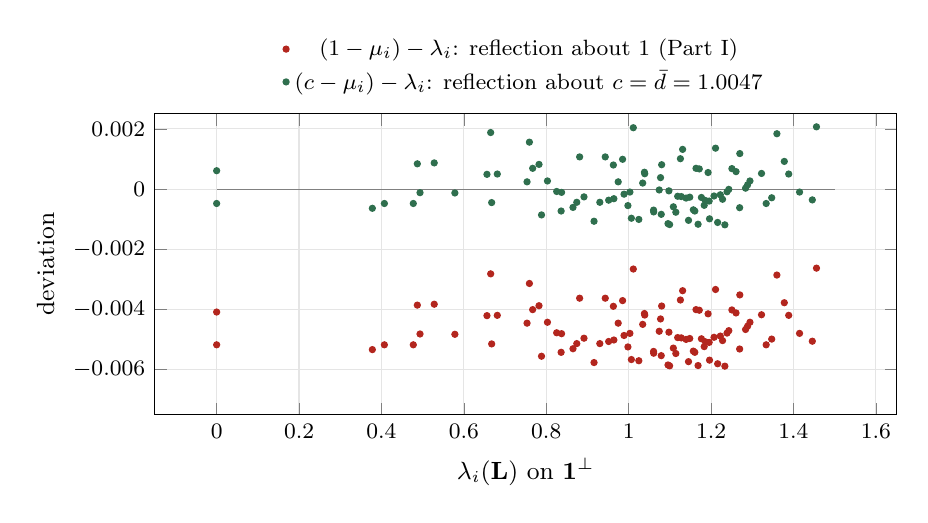
\begin{tikzpicture}
\begin{axis}[width=11cm,height=5.4cm,xlabel={$\lambda_i(\Lap)$ on $\one^\perp$},
  ylabel={deviation},
  legend style={at={(0.5,1.03)},anchor=south,font=\footnotesize,draw=none,fill=none,legend columns=1},
  tick label style={font=\footnotesize},label style={font=\small},
  scaled y ticks=false,yticklabel style={/pgf/number format/fixed,/pgf/number format/precision=3},
  ymin=-0.0075,ymax=0.0025,grid=major,grid style={gray!20}]
\addplot[gray,thin,forget plot] coordinates {(0,0) (1.5,0)};
\addplot[only marks,BadRed,mark=*,mark size=1.1pt] table[x=lam,y=dev] {
lam dev
0.0000 -0.00518
0.0000 -0.00409
0.3779 -0.00534
0.4071 -0.00518
0.4773 -0.00518
0.4871 -0.00386
0.4936 -0.00482
0.5281 -0.00383
0.5782 -0.00483
0.6561 -0.00421
0.6651 -0.00282
0.6675 -0.00515
0.6812 -0.00420
0.7534 -0.00446
0.7591 -0.00314
0.7670 -0.00401
0.7824 -0.00388
0.7885 -0.00556
0.8029 -0.00443
0.8253 -0.00478
0.8361 -0.00543
0.8372 -0.00481
0.8649 -0.00531
0.8741 -0.00514
0.8810 -0.00363
0.8916 -0.00496
0.9160 -0.00577
0.9300 -0.00514
0.9432 -0.00363
0.9515 -0.00507
0.9629 -0.00390
0.9641 -0.00502
0.9746 -0.00446
0.9853 -0.00371
0.9888 -0.00487
0.9982 -0.00525
1.0030 -0.00480
1.0066 -0.00567
1.0113 -0.00266
1.0247 -0.00571
1.0341 -0.00450
1.0383 -0.00414
1.0390 -0.00419
1.0605 -0.00540
1.0607 -0.00546
1.0742 -0.00473
1.0774 -0.00432
1.0791 -0.00554
1.0801 -0.00389
1.0955 -0.00585
1.0977 -0.00476
1.0994 -0.00588
1.1085 -0.00529
1.1145 -0.00547
1.1190 -0.00494
1.1256 -0.00369
1.1278 -0.00495
1.1310 -0.00338
1.1394 -0.00500
1.1453 -0.00574
1.1483 -0.00497
1.1570 -0.00539
1.1606 -0.00543
1.1635 -0.00401
1.1685 -0.00587
1.1714 -0.00403
1.1766 -0.00498
1.1834 -0.00524
1.1862 -0.00508
1.1928 -0.00415
1.1954 -0.00510
1.1963 -0.00569
1.2072 -0.00493
1.2109 -0.00334
1.2160 -0.00581
1.2225 -0.00489
1.2279 -0.00504
1.2335 -0.00589
1.2388 -0.00479
1.2431 -0.00471
1.2506 -0.00402
1.2606 -0.00412
1.2694 -0.00532
1.2698 -0.00352
1.2838 -0.00467
1.2887 -0.00456
1.2944 -0.00443
1.3225 -0.00418
1.3338 -0.00518
1.3472 -0.00499
1.3598 -0.00286
1.3778 -0.00378
1.3885 -0.00420
1.4148 -0.00480
1.4458 -0.00506
1.4559 -0.00263
};
\addlegendentry{$(1-\mu_i)-\lambda_i$: reflection about 1 (Part I)}
\addplot[only marks,LapC,mark=*,mark size=1.1pt] table[x=lam,y expr=\thisrow{dev}+0.0047] {
lam dev
0.0000 -0.00518
0.0000 -0.00409
0.3779 -0.00534
0.4071 -0.00518
0.4773 -0.00518
0.4871 -0.00386
0.4936 -0.00482
0.5281 -0.00383
0.5782 -0.00483
0.6561 -0.00421
0.6651 -0.00282
0.6675 -0.00515
0.6812 -0.00420
0.7534 -0.00446
0.7591 -0.00314
0.7670 -0.00401
0.7824 -0.00388
0.7885 -0.00556
0.8029 -0.00443
0.8253 -0.00478
0.8361 -0.00543
0.8372 -0.00481
0.8649 -0.00531
0.8741 -0.00514
0.8810 -0.00363
0.8916 -0.00496
0.9160 -0.00577
0.9300 -0.00514
0.9432 -0.00363
0.9515 -0.00507
0.9629 -0.00390
0.9641 -0.00502
0.9746 -0.00446
0.9853 -0.00371
0.9888 -0.00487
0.9982 -0.00525
1.0030 -0.00480
1.0066 -0.00567
1.0113 -0.00266
1.0247 -0.00571
1.0341 -0.00450
1.0383 -0.00414
1.0390 -0.00419
1.0605 -0.00540
1.0607 -0.00546
1.0742 -0.00473
1.0774 -0.00432
1.0791 -0.00554
1.0801 -0.00389
1.0955 -0.00585
1.0977 -0.00476
1.0994 -0.00588
1.1085 -0.00529
1.1145 -0.00547
1.1190 -0.00494
1.1256 -0.00369
1.1278 -0.00495
1.1310 -0.00338
1.1394 -0.00500
1.1453 -0.00574
1.1483 -0.00497
1.1570 -0.00539
1.1606 -0.00543
1.1635 -0.00401
1.1685 -0.00587
1.1714 -0.00403
1.1766 -0.00498
1.1834 -0.00524
1.1862 -0.00508
1.1928 -0.00415
1.1954 -0.00510
1.1963 -0.00569
1.2072 -0.00493
1.2109 -0.00334
1.2160 -0.00581
1.2225 -0.00489
1.2279 -0.00504
1.2335 -0.00589
1.2388 -0.00479
1.2431 -0.00471
1.2506 -0.00402
1.2606 -0.00412
1.2694 -0.00532
1.2698 -0.00352
1.2838 -0.00467
1.2887 -0.00456
1.2944 -0.00443
1.3225 -0.00418
1.3338 -0.00518
1.3472 -0.00499
1.3598 -0.00286
1.3778 -0.00378
1.3885 -0.00420
1.4148 -0.00480
1.4458 -0.00506
1.4559 -0.00263
};
\addlegendentry{$(c-\mu_i)-\lambda_i$: reflection about $c=\bar d=1.0047$}
\end{axis}
\end{tikzpicture}
\caption{How far each of the 96 eigenvalue pairs on $\one^\perp$ is from Part I's
prediction $\mu_i=1-\lambda_i$, on the repaired Fig.~2 graph (eigenvalues of $\Bmat$
taken in decreasing order, of $\Lap$ in increasing order). The offset of about
$-0.005$ is the mean degree's excess over one; once it is accounted for, what is left
is the spread of the degrees around their mean.}
\label{fig:spec}
\end{figure}

% =====================================================================
\section{Loosening the degree rule}\label{sec:sweep}
% =====================================================================

To see the match fail as degrees spread, I reran Algorithm 1 with the same data, $k$,
$\eta$ and start, lowering only the degree penalty $\rho$ (Table~\ref{tab:sweep}). The
rank constraint keeps holding: every run returns three components and no isolated
stock.

\begin{table}[h]
\centering\small
\footnotesize\setlength{\tabcolsep}{3pt}
\begin{tabular}{rcccccccc}
\toprule
$\rho$ & degree range & degree CV & components & rel.\ residual & $\mu_1,\mu_2$ of $\Bmat$ & $\sin$ & ARI vs comp.\ & $\mu_1,\mu_2$ of $\Bmat_n$ \\
\midrule
100 & [1.001, 1.007] & 0.0014 & 52/28/17 & 0.017 & 1.005, 1.004 & 0.002 & 1.000 & 1, 1 \\
30  & [1.004, 1.023] & 0.0047 & 52/28/17 & 0.056 & 1.017, 1.013 & 0.008 & 1.000 & 1, 1 \\
10  & [1.011, 1.064] & 0.0129 & 52/28/17 & 0.152 & 1.048, 1.038 & 0.021 & 1.000 & 1, 1 \\
3   & [1.031, 1.184] & 0.0344 & 52/28/17 & 0.392 & 1.139, 1.110 & 0.058 & 1.000 & 1, 1 \\
1   & [1.060, 1.421] & 0.0700 & 49/31/17 & 0.730 & 1.318, 1.254 & 0.123 & 1.000 & 1, 1 \\
0.3 & [1.109, 1.881] & 0.1265 & 52/28/17 & 1.098 & 1.647, 1.491 & 0.236 & 1.000 & 1, 1 \\
\bottomrule
\end{tabular}
\caption{Algorithm 1 at weaker degree penalties. Relative residual is
$\lVert\Bmat-(\Imat-\Lap-\one\one^\top/p)\rVert_F/\lVert\Bmat\rVert_F$; $\sin$ is the
largest principal angle between $\ker\Lap$ and $\operatorname{span}(\one,\text{top 2
of }\Bmat)$; ARI compares $k$-means on the top two eigenvectors of $\Bmat$ with the
components. The eigenvalues of $\Bmat_n$ equal 1 to six decimals in every row.}
\label{tab:sweep}
\end{table}

Three things stand out.
\begin{itemize}
\item \textbf{The algebra of Part I degrades steadily.} As the degree CV grows from
  $0.0014$ to $0.126$, the residual of \eqref{eq:B} grows from $1.7\%$ to more than the
  size of $\Bmat$ itself, the top eigenvalues of $\Bmat$ climb from $1.005$ to $1.65$,
  well past the ceiling of 1 in (a), and the subspaces drift apart.
\item \textbf{The normalised identity does not degrade at all.} $\Bmat_n$ keeps
  eigenvalue 1 with multiplicity exactly $k-1=2$ at every $\rho$, as
  Section~\ref{sec:classify} predicts for any degrees.
\item \textbf{The partition survives.} Even at $\rho=0.3$, $k$-means on the
  eigenvectors of the combinatorial $\Bmat$ returns the components exactly. With three
  components and no edges between them, the drift ($\sin\le0.24$) is not large enough
  to move any stock. I do not have a proof that this always happens; it is what these
  graphs show.
\end{itemize}

One run is out of line. At $\rho=1$ the components are 49/31/17: three Industrials
stocks, EFX, RSG and WM, join the Consumer Staples component (ARI against sectors
0.896). RSG and WM are waste-management companies, usually regarded as defensive, so
the grouping is plausible, but I have not tested it further; the runs at $\rho=3$ and
$\rho=0.3$ return the sectors exactly. It is a property of the learned graph, not of the Part I
comparison, which still matches the components exactly in that row.

% =====================================================================
\section{Scope of (c)}\label{sec:scope}
% =====================================================================

Part~(c) is exact under unit degree, but the paper's crash indicator comes from its
time-varying estimator, Problem (11), which has no degree constraint. As reported in
the 18 October note, our 243 learned FAAMUNG graphs have mean degree 2.13 and degree
CV 0.305, and $\lambda_2\ge1$ in 58\% of windows. On those graphs
$\lambda_{\max}(\Bmat_t)$ and $\lambda_2(\Lap_t)$ are different quantities, and the
sweep above shows how quickly the combinatorial match degrades once degrees spread
(the FAAMUNG CV is more than twice the largest in Table~\ref{tab:sweep}). I have
stated (c) for unit-degree graphs only. If a modularity indicator on the time-varying
graphs is still of interest, the normalised version
$\lambda_{\max}(\Bmat_n)=\max\{0,1-\lambda_2(\Lsym)\}$ holds for any degrees and could
be the version to test; whether that is worth doing is your call.

% =====================================================================
\section{Status of Part I}\label{sec:status1}
% =====================================================================

\begin{center}
\small
\begin{tabular}{>{\raggedright\arraybackslash}p{4.5cm}>{\raggedright\arraybackslash}p{2.4cm}>{\raggedright\arraybackslash}p{7.8cm}}
\toprule
claim & status & evidence \\
\midrule
(a) rank $\Leftrightarrow$ eigenvalue-1 multiplicity & proved; holds & Proposition~\ref{prop:lemma}; tests on 1 to 4 components; Fig.~2 graph gives $1.0052,1.0041$ (degree tolerance) \\
(b) Fan $=$ relaxed modularity & proved; holds under $\lambda_k\le1$ & exact form with $\max\{0,\lambda_k-1\}$; two counterexamples; Fig.~2 gap $0.0093$ \\
(c) $\mu_1=\max\{0,1-\lambda_2\}$ & proved; unit degree only & does not apply to Problem (11) graphs (Section~\ref{sec:scope}) \\
regular / normalised / unequal & proved & Table~\ref{tab:classify}; triangle-with-tails example; $\Bmat_n$ exact in every sweep run \\
$k$-means on $\Bmat$ recovers the components & reproduced & ARI 1.000 on Fig.~2 and at every $\rho$ \\
\bottomrule
\end{tabular}
\end{center}

\textbf{Deviations recorded.} The degree constraint is a quadratic penalty, so the
learned degrees are $1.0012$ to $1.0069$ rather than 1, and every spectral comparison
above carries that tolerance. The paper does not report $\eta$; $\eta=300$ is ours.
Algorithm 1 starts from the Problem (1) estimate, not the uniform graph (18 October
note). The $\rho$ sweep is ours, not the paper's.

\textbf{Reproducing.} \texttt{python report\_numbers.py -{}-part1} prints sections D to G of
its output from the committed caches in a few seconds; \texttt{python degree\_sweep.py 30 10 3 1
0.3} rebuilds the sweep; \texttt{tests/test\_lemma.py} (25 tests) checks the lemma, the
counterexamples and the classification on random graphs.

% =====================================================================
%  PART II
% =====================================================================
\clearpage
\begin{center}
{\Large\textbf{Part II: the market factor as an implicit null model}}
\end{center}
\vspace{1mm}

\newcommand{\Jmat}{\mathbf J}
\newcommand{\bvec}{\mathbf b}
\newcommand{\wvec}{\mathbf w}
\newcommand{\zvec}{\mathbf z}

% =====================================================================
\section{The implicit null}\label{sec:implicit}
% =====================================================================

Stock returns share a market factor, and modularity-based methods usually subtract an
explicit model of it (a null model) before looking for groups. The Laplacian learners
of the paper do not, and Part II asks whether they need to.

\begin{proposition}\label{prop:implicit}
Let $\Jmat=\Imat-\one\one^\top/p$. For every Laplacian $\Lap$ and every symmetric
$\Smat$, $\tr(\Lap\Smat)=\tr(\Lap\Jmat\Smat\Jmat)$. Hence Problem (1), Algorithm 1 and
any other estimator whose only data term is $\tr(\Lap\Smat)$ return the same graph from
$\Smat$ and from $\Jmat\Smat\Jmat$.
\end{proposition}
\begin{proof}
$\Lap\one=\mathbf 0$ gives $\Lap\Jmat=\Lap$, and by symmetry $\Jmat\Lap=\Lap$. So
$\tr(\Lap\Jmat\Smat\Jmat)=\tr(\Jmat\Lap\Jmat\Smat)=\tr(\Lap\Smat)$. The other terms of
these objectives (log-determinant, sparsity, degree, rank) depend on $\Lap$ alone.
\end{proof}

$\Jmat\Smat\Jmat$ is the covariance of the returns after each day's cross-sectional
average is subtracted. To see what that removes, take a one-factor model
$\Smat=\sigma^2\bvec\bvec^\top+\Smat_0$, where $\bvec$ holds the market loadings and
$\Smat_0$ the sector and idiosyncratic parts. The market's share of the data term is
\begin{equation}\label{eq:market}
  \tr(\Lap\,\sigma^2\bvec\bvec^\top)=\sigma^2\,\bvec^\top\Lap\bvec
  =\sigma^2\sum_{i<j}W_{ij}(b_i-b_j)^2 ,
\end{equation}
the usual Laplacian quadratic form. Two consequences follow.
\begin{itemize}
\item \textbf{Equal betas are removed exactly.} If $\bvec=c\one$, \eqref{eq:market} is
  zero for every graph: the learner ignores the market without any model of it.
\item \textbf{Unequal betas leave a penalty.} Otherwise the market charges every edge
  in proportion to the squared difference of the two stocks' betas, which pushes the
  graph to link stocks with similar betas. Equivalently, the learner sees the rank-one
  matrix $\sigma^2(\Jmat\bvec)(\Jmat\bvec)^\top$, which acts like an extra factor sorting
  stocks by beta. Its total size over all pairs is
  \[
    \sum_{i<j}(b_i-b_j)^2=p\sum_ib_i^2-\Big(\sum_ib_i\Big)^2=p\lVert\Jmat\bvec\rVert^2
    =p\lVert\bvec\rVert^2\sin^2\theta,
    \qquad
    \sin^2\theta=1-\frac{(\one^\top\bvec)^2}{p\lVert\bvec\rVert^2},
  \]
  where $\theta$ is the angle between $\bvec$ and $\one$. So $\sin^2\theta$ is the
  scale-free measure of how unequal the betas are, and the one used below.
\end{itemize}
Whether the penalty helps or hurts depends on how betas sit relative to the groups.
If stocks in the same sector have similar betas, it discourages exactly the edges
between sectors and reinforces the sectors. If betas vary inside sectors, it competes
with them.

Since the learners use the correlation matrix, the relevant loadings are
$b_i=\operatorname{corr}(x_i,f)$ rather than regression slopes; I call both ``betas''
where the difference does not matter and give both for the real data.

\textbf{Explicit nulls compared.} Four ways of removing the market before learning:
\begin{enumerate}[label=(\roman*)]
\item \emph{S-mode}: $\Smat-\mu_1\uvec_1\uvec_1^\top$, removing the top eigenmode,
  rescaled back to unit diagonal;
\item \emph{resid-SPX}: the correlation of the residuals after regressing each stock on
  the S\&P 500 index (\texttt{\^{}GSPC});
\item \emph{resid-EW}: the same, on the equal-weight average of the 97 stocks;
\item \emph{RMT}: the group component of MacMahon and Garlaschelli, the eigenmodes of
  $\Smat$ above the Marchenko-Pastur edge $(1+\sqrt{p/T})^2$ other than the market mode,
  with the unit diagonal put back.
\end{enumerate}
In the synthetic model there is also an \emph{oracle}: residuals on the true factor.

% =====================================================================
\section{A perturbation bound}\label{sec:bound}
% =====================================================================

The proposal asks for a bound linking unequal betas to the cluster eigenvectors. I give
it for Problem (1), which is convex; Algorithm 1 is not, and the argument below does not
apply to it. In the edge weights $\wvec=(W_{ij})_{i<j}\ge0$, the data term is
$\tr(\Lap\Smat)=\sum_{i<j}w_{ij}z_{ij}$ with $z_{ij}=S_{ii}+S_{jj}-2S_{ij}$, so Problem
(1) is
\[
  \min_{\wvec\ge0}\ \langle\wvec,\zvec(\Smat)+\gamma\one\rangle+g(\wvec),\qquad
  g(\wvec)=-\log\operatorname{gdet}\Lap(\wvec),
\]
with sparsity weight $\gamma$ (the paper's $\beta$; 10 here, the Fig.~1 setting). Adding
the market term $\bvec\bvec^\top$ to $\Smat$ adds $\Delta z_{ij}=(b_i-b_j)^2$ to
$\zvec$, a linear perturbation, with $\lVert\Delta\zvec\rVert_1=p\lVert\bvec\rVert^2
\sin^2\theta$. Let $\wvec_c$ be the solution for the clean matrix
$\Smat-\bvec\bvec^\top$ and $\wvec_o$ for the observed $\Smat$.

\begin{proposition}[Step 1]\label{prop:step1}
Suppose both solutions are connected graphs, and let $M$ be the larger of
$\lambda_{\max}(\Lap(\wvec_o))$ and $\lambda_{\max}(\Lap(\wvec_c))$. Then
\[
  \langle\Delta\zvec,\wvec_o-\wvec_c\rangle\le0,\qquad
  \lVert\wvec_o-\wvec_c\rVert\le\frac{M^2}{2}\lVert\Delta\zvec\rVert,\qquad
  \lVert\Lap(\wvec_o)-\Lap(\wvec_c)\rVert_F\le\sqrt{2p}\,\lVert\wvec_o-\wvec_c\rVert .
\]
\end{proposition}
\begin{proof}
\emph{Curvature.} For a connected $\Lap$ and a direction $\mathbf h$,
$\mathrm d^2g[\mathbf h,\mathbf h]=\tr(\Lap^+\Lap(\mathbf h)\Lap^+\Lap(\mathbf h))$. Since
$\Lap(\mathbf h)\one=\mathbf 0$, it acts on $\one^\perp$, where $\Lap^+\succeq
\lambda_{\max}^{-1}\Imat$, so the second derivative is at least
$\lVert\Lap(\mathbf h)\rVert_F^2/\lambda_{\max}^2$. Moreover
$\lVert\Lap(\mathbf h)\rVert_F^2=\sum_i(\sum_jh_{ij})^2+2\lVert\mathbf h\rVert^2\ge
2\lVert\mathbf h\rVert^2$. On the segment from $\wvec_c$ to $\wvec_o$ every graph is
connected, and $\lambda_{\max}$, being convex in $\wvec$, is at most $M$. So $g$ is
$\mu$-strongly convex there with $\mu=2/M^2$.

\emph{Comparison.} Optimality over $\wvec\ge0$ gives
$\langle\zvec+\Delta\zvec+\gamma\one+\nabla g(\wvec_o),\wvec_c-\wvec_o\rangle\ge0$ and
$\langle\zvec+\gamma\one+\nabla g(\wvec_c),\wvec_o-\wvec_c\rangle\ge0$. Adding them,
\[
  \mu\lVert\wvec_o-\wvec_c\rVert^2\le
  \langle\nabla g(\wvec_o)-\nabla g(\wvec_c),\wvec_o-\wvec_c\rangle\le
  \langle\Delta\zvec,\wvec_c-\wvec_o\rangle\le\lVert\Delta\zvec\rVert\,\lVert\wvec_o-\wvec_c\rVert .
\]
The middle inequality gives the sign statement, and dividing gives the second claim.
For the third, apply Cauchy-Schwarz to each row sum: $(\sum_jh_{ij})^2\le
(p-1)\sum_jh_{ij}^2$, and summing over $i$ gives at most $2(p-1)\lVert\mathbf h\rVert^2$;
adding $2\lVert\mathbf h\rVert^2$ gives $2p\lVert\mathbf h\rVert^2$.
\end{proof}

The sign statement has a plain reading: compared with the clean graph, the observed
graph has, in aggregate, moved weight away from pairs with different betas.

\textbf{Step 2} is the Davis-Kahan theorem in the form of Yu, Wang and Samworth (2015,
Theorem 2). Let $\Vmat_o,\Vmat_c$ hold the bottom $k$ eigenvectors of the two Laplacians
and $\mathrm{gap}=\lambda_{k+1}(\Lap_c)-\lambda_k(\Lap_c)>0$. Then
$\lVert\sin\Theta(\Vmat_o,\Vmat_c)\rVert_F\le2\sqrt k\,\lVert\Delta\Lap\rVert_2/\mathrm{gap}$.
Chaining the two steps through $\lVert\Delta\Lap\rVert_2\le\lVert\Delta\Lap\rVert_F$,
\begin{equation}\label{eq:chain}
  \lVert\sin\Theta\rVert_F\;\le\;\frac{\sqrt{2kp}\,M^2\,\lVert\Delta\zvec\rVert}{\mathrm{gap}},
  \qquad \lVert\Delta\zvec\rVert\le\lVert\Delta\zvec\rVert_1=p\lVert\bvec\rVert^2\sin^2\theta .
\end{equation}
This is the shape the proposal anticipated: the cluster subspace moves by at most a
constant times $\sin^2\theta/\mathrm{gap}$. Since $\lVert\sin\Theta\rVert_F\le\sqrt k$
always, \eqref{eq:chain} only says something when its right side is below $\sqrt k$.
Section~\ref{sec:boundcheck} checks each step against the learned graphs.

% =====================================================================
\section{Real data: the S\&P panel}\label{sec:real}
% =====================================================================

Same 97 stocks and 753 days as Part I; the index is \texttt{\^{}GSPC}, aligned to the
same days. The correlation loadings lie in $[0.177,\,0.743]$ (mean $0.513$), so
$\sin^2\theta=0.064$; the regression betas lie in $[0.347,\,1.839]$. The betas are
largely a sector attribute:

\begin{center}
\small
\begin{tabular}{lccc}
\toprule
 & Consumer Staples & Industrials & Energy \\
\midrule
mean loading & 0.363 & 0.597 & 0.506 \\
mean regression beta & 0.568 & 1.042 & 1.192 \\
\bottomrule
\end{tabular}
\end{center}
and $57.7\%$ of the variance of the loadings is between sectors. For the RMT null, the
Marchenko-Pastur edge is $1.847$ and 4 group modes lie above it.

Table~\ref{tab:real} shows both learners on all six inputs. The \emph{beta ratio}
measures the effect of \eqref{eq:market} inside sectors: it is the edge-weighted mean of
$|b_i-b_j|$ over within-sector pairs divided by the plain mean over the same pairs, so
values below 1 mean that within a sector the graph prefers to link stocks with similar
betas.

\begin{table}[h]
\centering\small
\begin{tabular}{lccccccc}
\toprule
 & \multicolumn{4}{c}{Algorithm 1 ($k=3$)} & \multicolumn{3}{c}{Problem (1) + $k$-means} \\
\cmidrule(lr){2-5}\cmidrule(lr){6-8}
input & comp. & ARI sectors & ARI beta & beta ratio & ARI sectors & ARI beta & beta ratio \\
\midrule
$\Smat$ (implicit null) & 3 & \textbf{1.000} & 0.277 & 0.786 & \textbf{0.900} & 0.295 & 0.862 \\
$\Jmat\Smat\Jmat$ & 3 & 1.000 & 0.277 & 0.786 & 0.900 & 0.295 & 0.862 \\
\midrule
S-mode & 1 & 0.830 & 0.257 & 0.820 & 0.867 & 0.292 & 0.879 \\
resid-SPX & 1 & 0.830 & 0.257 & 0.816 & 0.802 & 0.252 & 0.872 \\
resid-EW & 3 & 0.896 & 0.298 & 0.794 & 0.867 & 0.292 & 0.867 \\
RMT & 1 & 0.875 & 0.291 & 0.928 & 0.900 & 0.268 & 0.944 \\
\bottomrule
\end{tabular}
\caption{The S\&P panel. ``comp.'' is the number of connected components Algorithm 1
returns; where it is 1, the clusters come from $k$-means on the bottom three
eigenvectors (spectral fallback). ARI beta compares the clusters with terciles of the
loadings.}
\label{tab:real}
\end{table}

\begin{itemize}
\item \textbf{The invariance holds numerically.} The graphs learned from $\Smat$ and
  $\Jmat\Smat\Jmat$ agree to $2.7\times10^{-10}$ (Problem (1)) and $1.3\times10^{-4}$
  (Algorithm 1, within its stopping tolerance), and every metric is identical.
\item \textbf{No explicit null does better than the implicit one.} Under Algorithm 1
  every explicit null loses: ARI 0.830 to 0.896 against 1.000. Under Problem (1) the RMT
  null ties (0.900) and the others lose (0.802 to 0.867).
\item \textbf{A likely reason is that betas carry sector information here.} With
  $57.7\%$ of the loading variance between sectors, the penalty \eqref{eq:market} falls
  mostly on edges between sectors and so supports the sector split. Removing the market
  removes that support. This is the ``aligned'' case of Section~\ref{sec:synthetic},
  where unequal betas never hurt.
\item \textbf{The penalty is visible inside sectors.} On $\Smat$ the beta ratio is
  0.786 (Algorithm 1) and 0.862 (Problem (1)). Every explicit null raises it, RMT most
  (0.928, 0.944), as \eqref{eq:market} predicts once the market term is gone. The
  market term is small in absolute terms: $\bvec^\top\Lap\bvec$ is $1.1\%$ of
  $\tr(\Lap\Smat)$ on the Algorithm 1 graph and $1.7\%$ on the Problem (1) graph.
\end{itemize}
Algorithm 1 did not reach three components on three of the four explicit nulls within
its 80 outer iterations (Table~\ref{tab:real}); with $\Smat$ it does. I recorded this
as a deviation and used the spectral fallback rather than tuning the solver per input.

% =====================================================================
\section{Synthetic data: when betas cut across sectors}\label{sec:synthetic}
% =====================================================================

\textbf{Model.} $x_{t,i}=b_if_t+s_{g(i),t}+e_{t,i}$ with independent Gaussian market
$f_t\sim N(0,1)$, sector factors $s_{g,t}\sim N(0,0.6^2)$ and noise
$e_{t,i}\sim N(0,1.2^2)$; $p=60$ stocks in three sectors of 20 and $T=753$ days, as in
the real panel. Three beta designs:
\begin{itemize}
\item \emph{equal}: every $b_i=1$;
\item \emph{aligned}: $b_i=1-\delta,\ 1,\ 1+\delta$ by sector, so betas follow sectors;
\item \emph{cross}: in every sector, half the stocks at $1+\delta$ and half at
  $1-\delta$, so the beta split is orthogonal to the sectors.
\end{itemize}
The population correlation loadings are $b_i/\sqrt{b_i^2+0.6^2+1.2^2}$, and
$\sin^2\theta$ below is computed from them. Each run learns from $\Smat$, from S-mode
and from the oracle, with both learners.

\textbf{Coarse grid} ($\delta=0.2,0.4,0.6,0.8$, seeds 0 and 1; 108 runs).
\begin{itemize}
\item \emph{Equal and aligned}: every input and learner recovers the sectors exactly
  (ARI 1.000) in every run, up to $\sin^2\theta=0.219$ (aligned, $\delta=0.8$). Unequal
  betas are harmless when they follow the groups.
\item \emph{Cross}: at $\delta=0.2$ and 0.4 ($\sin^2\theta=0.017$, 0.072) everything
  is still exact. At $\delta=0.6$ and 0.8 ($\sin^2\theta=0.173$, 0.322), both learners
  on $\Smat$ cluster by beta in both seeds: ARI 0.134 against the sectors and 0.773
  against the two beta groups (not 1, because there are three clusters for two
  groups). S-mode and the oracle stay at 1.000.
\end{itemize}

\textbf{Fine grid} (cross design, $\delta$ from 0.400 to 0.600 in steps of 0.025, seeds 0
to 4; 270 runs) locates the switch (Table~\ref{tab:threshold},
Figure~\ref{fig:threshold}). S-mode and the oracle give ARI 1.000 against the sectors
in all 180 of their runs.

\begin{table}[h]
\centering\small
\begin{tabular}{cccccc}
\toprule
 & & \multicolumn{2}{c}{Algorithm 1 on $\Smat$} & \multicolumn{2}{c}{Problem (1) on $\Smat$} \\
\cmidrule(lr){3-4}\cmidrule(lr){5-6}
$\delta$ & $\sin^2\theta$ & ARI sectors & seeds by beta & ARI sectors & seeds by beta \\
\midrule
0.400 & 0.0715 & 1.000 & 0/5 & 1.000 & 0/5 \\
0.425 & 0.0815 & 1.000 & 0/5 & 1.000 & 0/5 \\
0.450 & 0.0921 & 1.000 & 0/5 & 1.000 & 0/5 \\
0.475 & 0.1036 & 1.000 & 0/5 & 1.000 & 0/5 \\
0.500 & 0.1158 & 1.000 & 0/5 & 0.767 & 1/5 \\
0.525 & 0.1288 & 1.000 & 0/5 & 0.346 & 3/5 \\
0.550 & 0.1426 & 0.767 & 1/5 & 0.134 & 5/5 \\
0.575 & 0.1572 & 0.459 & 2/5 & 0.134 & 5/5 \\
0.600 & 0.1726 & 0.134 & 5/5 & 0.134 & 5/5 \\
\bottomrule
\end{tabular}
\caption{The switch from sectors to beta groups, cross design. ARI sectors is the mean
over 5 seeds; ``seeds by beta'' counts the seeds whose clusters match the beta groups
better than the sectors.}
\label{tab:threshold}
\end{table}

\begin{figure}[h]
\centering
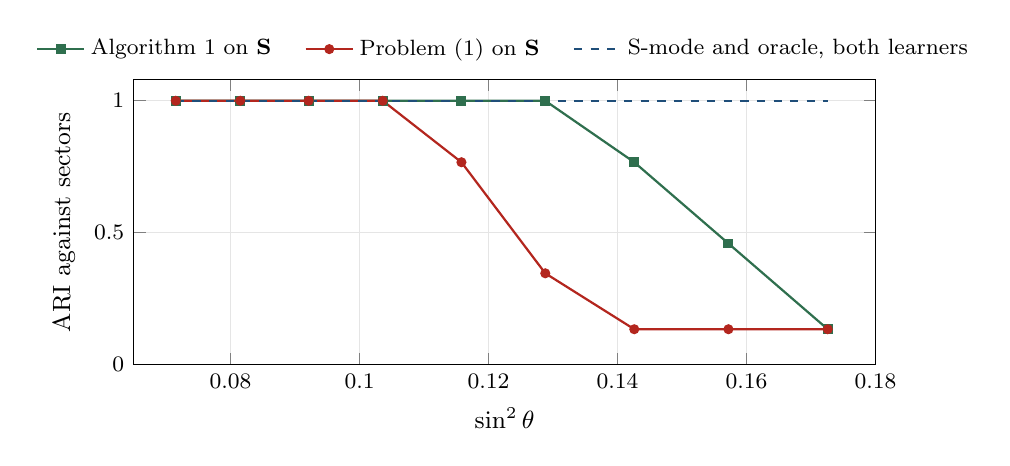
\begin{tikzpicture}
\begin{axis}[width=11cm,height=5.2cm,xlabel={$\sin^2\theta$},ylabel={ARI against sectors},
  legend style={at={(0.5,1.03)},anchor=south,font=\footnotesize,draw=none,fill=none,legend columns=3,
    /tikz/every even column/.append style={column sep=10pt}},
  tick label style={font=\footnotesize},label style={font=\small},
  xmin=0.065,xmax=0.18,ymin=0,ymax=1.08,grid=major,grid style={gray!20},
  xticklabel style={/pgf/number format/fixed,/pgf/number format/precision=2}]
\addplot[LapC,thick,mark=square*,mark size=1.4pt] coordinates {
(0.0715,1.000) (0.0815,1.000) (0.0921,1.000) (0.1036,1.000) (0.1158,1.000)
(0.1288,1.000) (0.1426,0.767) (0.1572,0.459) (0.1726,0.134)};
\addlegendentry{Algorithm 1 on $\Smat$}
\addplot[BadRed,thick,mark=*,mark size=1.4pt] coordinates {
(0.0715,1.000) (0.0815,1.000) (0.0921,1.000) (0.1036,1.000) (0.1158,0.767)
(0.1288,0.346) (0.1426,0.134) (0.1572,0.134) (0.1726,0.134)};
\addlegendentry{Problem (1) on $\Smat$}
\addplot[BlueLink,thick,dashed] coordinates {(0.0715,1.0) (0.1726,1.0)};
\addlegendentry{S-mode and oracle, both learners}
\end{axis}
\end{tikzpicture}
\caption{Mean ARI against the sectors over 5 seeds, cross design. The implicit null
switches to clustering by beta over a narrow range of $\sin^2\theta$; the explicit nulls
never do.}
\label{fig:threshold}
\end{figure}

The switch is sharp. For Problem (1) it begins between $\sin^2\theta=0.104$ and
$0.116$ and is complete by $0.143$; for Algorithm 1 it begins between $0.129$ and $0.143$
and is complete by $0.173$. Algorithm 1 holds out longer; I have not tested why. The
location depends on the strength of the sector factor relative to the noise, which
here is our choice ($0.6$ against $1.2$), so these values are specific to this design.
The real panel's $\sin^2\theta=0.064$ is not directly comparable for that reason;
Section~\ref{sec:boundcheck} gives a comparison that does transfer.

% =====================================================================
\section{The bound against the measurements}\label{sec:boundcheck}
% =====================================================================

Table~\ref{tab:bound} evaluates each step of Section~\ref{sec:bound} for Problem (1) on
the cross design (mean over seeds 0 to 2) and on the real panel. The clean graph is
learned from $\Smat-\bvec\bvec^\top$ with the population loadings (synthetic) or the
sample loadings on \texttt{\^{}GSPC} (real). $M$ is between 0.189 and 0.195 in every
row.

\begin{table}[h]
\centering\footnotesize\setlength{\tabcolsep}{3pt}
\begin{tabular}{ccccccccccccc}
\toprule
 & & \multicolumn{3}{c}{Step 1: $\lVert\Delta\wvec\rVert$} & \multicolumn{2}{c}{$\lVert\Delta\Lap\rVert$} & & & & \multicolumn{2}{c}{Step 2: DK} & \\
\cmidrule(lr){3-5}\cmidrule(lr){6-7}\cmidrule(lr){11-12}
$\delta$ & $\sin^2\theta$ & actual & bound & ratio & 2-norm & F bound & gap & $\dfrac{\lVert\Delta\Lap\rVert_2}{\mathrm{gap}}$ & $\lVert\sin\Theta\rVert_F$ & actual $\Delta\Lap$ & chain & ARI \\
\midrule
0.20 & 0.017 & 0.0078 & 0.0129 & 1.65 & 0.0111 & 0.141 & 0.0451 & 0.247 & 0.007 & 0.86 & 10.9 & 1.00 \\
0.30 & 0.039 & 0.0164 & 0.0296 & 1.80 & 0.0234 & 0.324 & 0.0443 & 0.528 & 0.022 & 1.83 & 25.4 & 1.00 \\
0.40 & 0.072 & 0.0268 & 0.0540 & 2.02 & 0.0381 & 0.592 & 0.0435 & 0.877 & 0.070 & 3.04 & 47.2 & 1.00 \\
0.45 & 0.092 & 0.0322 & 0.0693 & 2.15 & 0.0459 & 0.759 & 0.0430 & 1.067 & 0.147 & 3.70 & 61.2 & 1.00 \\
0.50 & 0.116 & 0.0377 & 0.0868 & 2.30 & 0.0537 & 0.951 & 0.0425 & 1.263 & 0.375 & 4.38 & 77.6 & 0.73 \\
0.55 & 0.143 & 0.0431 & 0.1067 & 2.47 & 0.0614 & 1.169 & 0.0420 & 1.464 & 0.947 & 5.08 & 96.6 & 0.13 \\
0.60 & 0.173 & 0.0484 & 0.1290 & 2.67 & 0.0689 & 1.413 & 0.0413 & 1.668 & 0.984 & 5.78 & 118.6 & 0.13 \\
0.80 & 0.322 & 0.0673 & 0.2445 & 3.63 & 0.0957 & 2.678 & 0.0381 & 2.509 & 0.994 & 8.70 & 243.5 & 0.13 \\
\midrule
real & 0.064 & 0.0156 & 0.0756 & 4.84 & 0.0212 & 1.053 & 0.0317 & 0.669 & 0.157 & 2.32 & 114.9 & 0.90 \\
\bottomrule
\end{tabular}
\caption{Problem (1). ``ratio'' is the Step 1 bound over the actual movement;
``2-norm'' is the actual $\lVert\Delta\Lap\rVert_2$; the $\lVert\Delta\Lap\rVert_F$ bound is $\sqrt{2p}$ times the Step 1 bound; ``DK, actual
$\Delta\Lap$'' is $2\sqrt k\lVert\Delta\Lap\rVert_2/\mathrm{gap}$ with the true
$\Delta\Lap$; ``chain'' is \eqref{eq:chain}. Any DK value above
$\sqrt k=1.732$ is vacuous. ARI is that of the observed graph against the sectors; the
clean graph scores 1.00 in every synthetic row and 0.87 on the real data.}
\label{tab:bound}
\end{table}

\begin{itemize}
\item \textbf{Step 1 is valid and fairly tight.} The bound on $\lVert\Delta\wvec\rVert$
  exceeds the actual movement by a factor 1.65 to 3.63 on the synthetic grid (2.15 to
  2.47 around the switch) and 4.84 on the real data.
\item \textbf{Passing to $\Delta\Lap$ loses a further factor of about 8.} At
  $\delta=0.5$ the actual $\lVert\Delta\Lap\rVert_F/\lVert\Delta\wvec\rVert$ is 1.43,
  against the worst case $\sqrt{2p}=10.95$: the weight changes are spread over many
  edges and their row sums largely cancel.
\item \textbf{Step 2 is vacuous here, even with the true $\Delta\Lap$.} The eigengap of
  the clean graph is only about 0.04, so $2\sqrt k\lVert\Delta\Lap\rVert_2/\mathrm{gap}$
  passes $\sqrt k$ already at $\delta=0.3$, where the subspace has moved by 0.022.
  The full chain \eqref{eq:chain} gives 10.9 to 243.5, against a maximum possible
  value of 1.732.
\item \textbf{The ratio $\lVert\Delta\Lap\rVert_2/\mathrm{gap}$ does locate the switch.}
  At 0.877 and 1.067 nothing has switched ($\lVert\sin\Theta\rVert_F$ 0.070 and
  0.147); at 1.263 one seed in three has switched (0.375); at 1.464 all have (0.947).
  So the switch happens when the perturbation reaches about the eigengap, which is the
  scale Davis-Kahan names, but its constant 2 and the slack in Step 1 put the
  certified threshold far below the real one.
\item \textbf{On the real data the ratio is 0.669}, below every synthetic row that
  switched. This comparison does not depend on the sector strength, since both the
  perturbation and the gap are measured on the data, and it agrees with the finding
  that the implicit null suffices there. It is a measured rule on one design and one
  learner, not a theorem.
\end{itemize}

% =====================================================================
\section{Status of Part II}\label{sec:status2}
% =====================================================================

\begin{center}
\small
\renewcommand{\arraystretch}{1.2}
\begin{tabular}{>{\raggedright\arraybackslash}p{4.8cm}>{\raggedright\arraybackslash}p{2.6cm}>{\raggedright\arraybackslash}p{7.3cm}}
\toprule
claim & status & evidence \\
\midrule
$\tr(\Lap\Smat)=\tr(\Lap\Jmat\Smat\Jmat)$ & proved; reproduced & Proposition~\ref{prop:implicit}; graphs agree to $2.7\times10^{-10}$ and $1.3\times10^{-4}$ \\
market term penalises edges between different betas, total size $\propto\sin^2\theta$ & proved & \eqref{eq:market}; unit tests \\
implicit null suffices on the S\&P panel & holds & Algorithm 1 ARI 1.000 from $\Smat$ \\
explicit null improves on it (real data) & \textbf{not supported} & Algorithm 1: 0.830 to 0.896; Problem (1): 0.802 to 0.900 (RMT ties) \\
unequal betas aligned with groups are harmless & reproduced (synthetic) & ARI 1.000 in every aligned run, up to $\sin^2\theta=0.219$ \\
cross-cutting betas break the implicit null & reproduced (synthetic) & switch at $\sin^2\theta$ 0.116 to 0.143 (Problem (1)), 0.143 to 0.173 (Algorithm 1) \\
explicit nulls fix that & reproduced (synthetic) & ARI 1.000 in all 180 fine-grid runs and all coarse-grid runs \\
Step 1 bound & proved; holds & within a factor 1.65 to 4.84 \\
Davis-Kahan chain & proved; \textbf{vacuous} & 10.9 to 243.5 against a ceiling of 1.732 \\
switch when $\lVert\Delta\Lap\rVert_2\approx\mathrm{gap}$ & observed, not proved & no switch at 1.067, partial at 1.263; real data 0.669 \\
\bottomrule
\end{tabular}
\end{center}

\textbf{Deviations recorded.}
\begin{itemize}
\item The index is \texttt{\^{}GSPC} from Yahoo Finance; the paper does not use one.
\item S-mode is rescaled to unit diagonal, and RMT has its unit diagonal put back, so
  that both are correlation-like inputs.
\item Algorithm 1 ends with a single component on three real inputs (S-mode,
  resid-SPX, RMT) and on one synthetic run (aligned, $\delta=0.2$, seed 1, $\Smat$,
  where $\lambda_2=\lambda_3=0.0033$). These use the spectral fallback; the synthetic one
  still scores 1.000. None of the 135 fine-grid Algorithm 1 runs needed it.
\item The bound is for Problem (1) only, as Algorithm 1 is not convex.
\item Synthetic $\sin^2\theta$ uses population loadings and real $\sin^2\theta$ sample
  loadings. The synthetic variances are ours, and the switch location depends on them.
\item As in Part I, $\eta=300$, $\rho=100$ and the start are ours; Problem (1) uses
  sparsity 10 as in Fig.~1.
\end{itemize}

\textbf{Reproducing.} \texttt{python report\_numbers.py -{}-part2} prints sections H to L
from the caches in \texttt{part2\_cache/} in a few seconds (section L relearns its
Problem (1) graphs). \texttt{python part2\_runs.py WORKER} rebuilds the 120 main runs
(about 45 minutes with two workers) and \texttt{python part2\_threshold.py} the fine
grid; \texttt{tests/test\_part2.py} (9 tests) checks the invariance, the identity
\eqref{eq:market} and the generator.

\textbf{Next.} Two possible directions, for you to decide between.
\begin{itemize}
\item \emph{Part III} can start once you choose a repair for its objective (18 October
  note). Parts I and II together suggest what it should aim at: under unit degree
  modularity adds nothing, and on this panel the implicit null already does the job,
  so a gain would have to come from unequal degrees.
\item \emph{Part II on harder data.} The S\&P panel is the easy case because betas
  follow sectors. A universe where betas vary strongly within sectors (for example a
  broader cross-section of the S\&P 500) would test whether the switch seen in the
  synthetic data happens in practice, with the ratio
  $\lVert\Delta\Lap\rVert_2/\mathrm{gap}$ as the diagnostic.
\end{itemize}

\end{document}
